\section{System}
\label{sec:system}

In this section we give an high level description of the target system.

% %
% SYSTEM DESCRIPTION
% %
We consider the environment in Figure~\ref{fig:system-architecture}, which is characterized by:

\begin{itemize}
	\item  \textbf{workload:} mobile devices send to the system tasks partitioned in two classes.
	\item \textbf{system:} a two-layers Fog-like system, made of:	
	\begin{itemize}
		\item \textbf{Cloudlet:} upfront layer made of one-hop finite resources, having the ability to off-load tasks to the Cloud server, accordingly to an \textit{off-loading policy} based on the occupancy state of the Cloudlet. In particular, the Cloudlet may \textit{forward} incoming tasks to Cloud or \textit{restart} preempted tasks in Cloud with some \textit{overhead}.
		\item \textbf{Cloud:} backfront layer made of a remote Cloud server with virtually unlimited resources.
		
	\end{itemize}
\end{itemize}

We assume that
(i) the Cloudlet provides tasks with higher service rate than the Cloud, 
(ii) when a task is interrupted in the Cloudlet and it is sent to the Cloud, the restart process comes with a \textit{setup time overhead}.

\begin{figure}
	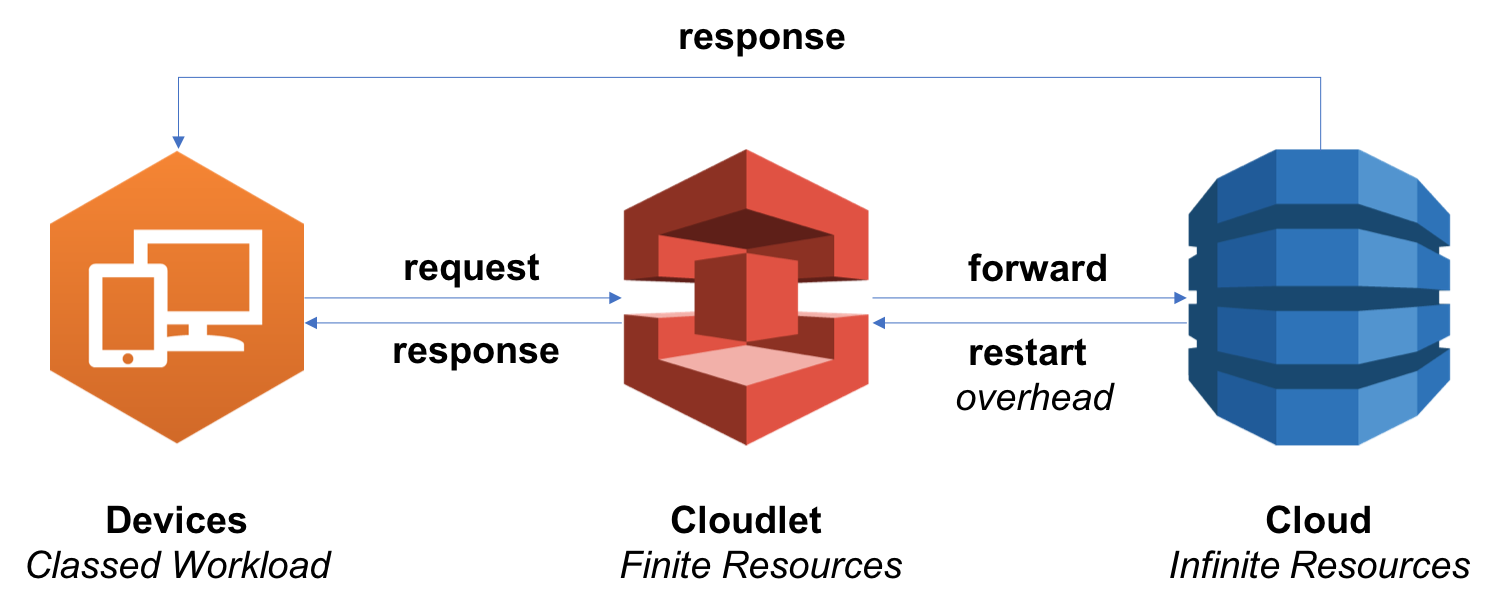
\includegraphics[width=\columnwidth]{fig/system-architecture}
	\caption{System architecture (high level).}
	\label{fig:system-architecture}
\end{figure}

Such a system can be considered very actual nowadays. In fact, it sketches the typical asset of a simple Fog Computing solution.